% =====================================================================
%  Chapter 4 - Implementation
%  Rewritten 2026-08-05. Expanded to match the 25% rubric weight:
%  adds codebase structure + module table, gate pseudocode, an explicit
%  testing strategy, the demo interface, and a maintainability section.
%  All previous labels preserved so cross-references from other chapters
%  continue to resolve.
% =====================================================================
\chapter{Implementation}
\label{ch:impl}

\section{Codebase Structure}
\label{sec:impl-structure}

The system is implemented as a single installable Python package,
\texttt{medrag\_adaptive}, in which the six design layers of
Section~\ref{sec:method-overview} are realised as the subpackages of
Table~\ref{tab:impl-modules}, together with driver scripts that sit outside
the package and do nothing except orchestrate. Keeping the drivers outside is
deliberate, because an experiment's identity is a combination of configuration
files, index paths and an output log rather than a piece of code, so nothing
inside the package ever needs to know which experiment is running.

\begin{table}[t]
  \centering
  \small
  \begin{tabular}{@{}lll@{}}
    \toprule
    Subpackage & Responsibility & Representative modules \\
    \midrule
    \texttt{config} & layered YAML merge and validation & \texttt{config.py} \\
    \texttt{data} & loaders, unified schema, risk tagging & \texttt{schema.py}, \texttt{risk\_tagger.py} \\
    \texttt{models} & inference backends and prompt construction & \texttt{llama\_backend.py}, \texttt{prompts.py} \\
    \texttt{retrieval} & BM25, dense and hybrid retrievers & \texttt{hybrid\_retriever.py} \\
    \texttt{gating} & three gates and the majority-vote ensemble & \texttt{entropy\_gate.py}, \texttt{ensemble\_gate.py} \\
    \texttt{policies} & P1--P5 and the hardware-aware factory & \texttt{p5\_gated.py}, \texttt{factory.py} \\
    \texttt{evaluation} & scorers, profiler, canonical log loader & \texttt{scoring.py}, \texttt{loading.py} \\
    \texttt{ui} & demonstration interface and its renderers & \texttt{session.py}, \texttt{attribution.py} \\
    \bottomrule
  \end{tabular}
  \caption{Package layout. Each subpackage depends only on those above it and
  communicates through the typed dataclasses of Section~\ref{sec:impl-config},
  which is what allows any layer to be tested against mock collaborators.}
  \label{tab:impl-modules}
\end{table}

Each subpackage depends only on those above it and all traffic between them
passes through the shared dataclasses described below, so the gating layer,
which is both the novel part of the project and the part most likely to
change, was built last against a substrate already covered by tests. When the
verbalized-confidence gate of the original design was replaced by the
hallucination probe (Section~\ref{sec:method-gates}), the change touched one
new module and one configuration entry, and no policy, retriever or scorer
required editing.

\section{Configuration and Data Contracts}
\label{sec:impl-config}

Every experiment in this study is a point in a space of hardware tier
$\times$ model $\times$ retrieval policy $\times$ dataset, and hard-coding
those combinations would produce many near-duplicate scripts and make any
reproducibility claim difficult to audit. Configuration is instead expressed
as YAML files deep-merged in increasing precedence,
\[
  \texttt{base} \rightarrow \texttt{hardware} \rightarrow \texttt{model}
  \rightarrow \texttt{policy} \rightarrow \texttt{experiment},
\]
so that a later file overrides only the keys it actually names. The merged
dictionary is then validated into a typed \texttt{ProjectConfig} using
Pydantic before any expensive computation begins, which matters a great deal
when a single run occupies several hours of CPU time and a typo in a
threshold would otherwise only surface at the end of it.

The \texttt{logits\_all} flag is the clearest example of a design decision
being encoded declaratively rather than in code. The entropy and margin gates
need the model's per-token logit distribution, which the inference library
retains only when the model is constructed with \texttt{logits\_all=true}, at
a memory cost of roughly 256\,MB. The low hardware tier overrides that flag to
\texttt{false}, which automatically renders both logit gates unavailable and
forces the ensemble into the probe-only degraded mode of
Section~\ref{sec:method-ensemble}. The hardware trade-off is therefore
readable from the configuration alone, and there is no runtime conditional
buried in the gating code that a reader would have to discover.

Communication between layers passes through three dataclasses held in a
dependency-free schema module. \texttt{UnifiedQuestion} normalises any source
dataset into one shape, carrying a \texttt{choices} mapping and gold letter
for multiple-choice items, a gold answer string for open-ended ones, and a
tagger-assigned \texttt{risk\_level} on every question.
\texttt{PolicyResult} is one policy's output on one question, holding the
answer text, the gate decision and its signals, the retrieved chunks and the
profiling fields. \texttt{RunRecord} adds ground-truth scoring and experiment
metadata and is serialised as one JSON Lines record per query.

That append-only JSONL log is central to both resumability and analysis.
Because each line is independent of the others, an interrupted run resumes by
reading back the \texttt{question\_id}s already present and skipping them,
which is what makes multi-hour experiments practical on a laptop that may
sleep or be closed. Each record also carries a free-form \texttt{qvault}
dictionary holding the gate-specific payloads, namely the per-token entropy
array, both probe drafts, the per-member votes and the retrieved chunk texts,
which can grow without any schema change. This is what later allowed every
analysis in Chapter~\ref{ch:eval}, including the calibration sweeps, the
ablations and the paired distraction study, to be replayed offline from the
logs without invoking the model again.

The clinical-risk tagger assigns each question a level in
$\{\text{low}, \text{medium}, \text{high}\}$ using a keyword rule set with
precedence $\textsc{high} \succ \textsc{low} \succ \textsc{medium}$ and a
conservative default of \textsc{medium}, the high-risk cues being dosing,
overdose, drug interactions, contraindications and acute emergencies. A rule
set was chosen over a learned classifier because in a safety context the basis
of each label has to be inspectable, and because no labelled training data
exists for the task.

\section{Model Backend and Prompting}
\label{sec:impl-backend}

The language model is served entirely on CPU by a backend wrapping
\texttt{llama.cpp} \citep{llamacpp}, running Llama-3.2-3B-Instruct
\citep{llama3} at 4-bit quantisation (Q4\_K\_M, GGUF). Determinism is enforced
by greedy decoding at temperature 0 with a fixed seed, and the configuration
validator warns if a non-zero temperature is ever supplied, since that would
silently break reproducibility without failing anything.

Two backend methods exist purely to serve the gates. \texttt{draft()} returns
the generated text together with the raw logit array of shape
$[n_{\text{gen}} \times |V|]$, which is the entropy gate's input, while
\texttt{get\_top2\_logprobs()} returns per-position top-two log-probabilities
through the completion API rather than the logit buffer, which is what allows
the margin gate to survive \texttt{logits\_all=false}. Both are declared on
the abstract backend interface, so a \texttt{MockLLMBackend} can supply
deterministic text and synthetic logit arrays in their place, which is what
the entire model-free test suite rests on.

Prompt construction separates the message bodies from the chat-template
wrapper, with a single \texttt{set\_chat\_format()} call at backend
construction selecting \texttt{llama}, \texttt{qwen} or \texttt{plain}. No
policy or gate is able to assemble a prompt in the wrong format for the loaded
model, because none of them ever sees the wrapper. This refactor was the
riskiest change made to the codebase, since it could have silently invalidated
every result already collected, so it was verified to produce byte-identical
prompts for all eight prompt types under the default Llama format before being
merged, which is why the existing Llama-3.2-3B logs remained valid afterwards.
It is also the mechanism through which the scaling study of
Chapter~\ref{ch:scaling} ran without any change to policy or gate code, as the
Qwen2.5-7B and 14B experiments altered only the model file, the chat format
and the calibrated thresholds.

\section{Implementing the Gate Ensemble}
\label{sec:impl-gating}

Each gate implements one method, \texttt{decide(question, llm)}, returning a
\texttt{GateDecision} that carries a boolean, the raw signal value and a
details dictionary. The details dictionary is where the availability flag
lives, and the ensemble reads it to decide whether a member is entitled to
vote at all. Listing~\ref{lst:ensemble} gives the decision procedure.

\begin{lstlisting}[language=Python, caption={Ensemble decision with
availability accounting and degraded-mode fallback.},
label={lst:ensemble}]
def decide(question, llm):
    retrieve_votes = 0
    available      = 0
    votes, signals = {}, {}

    for member in self.members:
        d = member.decide(question, llm)
        if not d.details.get("available", True):
            votes[member.name] = "abstain"   # excluded from the electorate
            continue
        available += 1
        signals[member.name] = d.signal_value
        votes[member.name]   = d.decision_str
        retrieve_votes += int(d.retrieve)

    degraded = available < self.min_votes
    retrieve = (retrieve_votes >= 1) if degraded \
               else (retrieve_votes >= self.min_votes)

    return GateDecision(retrieve=retrieve,
                        details={"votes": votes, "signals": signals,
                                 "members_available": available,
                                 "degraded": degraded, ...})
\end{lstlisting}

Two properties of this procedure are worth drawing out. The first is that an
abstaining member is removed from the electorate rather than counted as a vote
to skip, which is the difference between a gate that is unavailable and a gate
that is confident, and conflating the two would have biased the low hardware
tier toward never retrieving. The second is that the degraded branch is
reached by counting availability rather than by inspecting the hardware tier,
so the fallback is a property of what actually loaded rather than of what the
configuration claimed. The policy factory reinforces this at construction
time, inspecting the backend's \texttt{logits\_all} setting and downgrading a
requested three-gate ensemble to probe-only when the logit buffer is disabled,
so a configuration cannot request a gate the hardware cannot support. Every
one of these fields is written into the JSONL record, which is what makes the
gate ablation of Section~\ref{sec:eval-ablation} a replay over logged votes
rather than a re-run.

\section{Corpus Construction and Indexing}
\label{sec:impl-corpus}

The evaluation initially used a 200-chunk pilot corpus, which produced the
corpus-bottleneck finding of Section~\ref{sec:eval-corpus} and forced a real
corpus build. Verifying dataset paths before committing to them, a habit
acquired when the originally planned open-ended dataset proved unreachable at
its published location, revealed that the StatPearls sub-corpus was empty on
the hosting hub while the MedRAG textbooks ($\sim$126K snippets) and PubMed
corpora resolved correctly. The corpus was therefore assembled from the
medical textbooks plus a 300,000-snippet PubMed slice, giving
\textbf{425,847 chunks}, roughly $2{,}100\times$ the pilot.

Embedding 426K chunks on a memory-constrained CPU laptop required a build that
survives interruption, because a single uninterrupted run of that length could
not be relied on. The build script embeds in fixed shards of 2,000 and
checkpoints each shard to disk, so a crash or a process kill loses at most one
shard of work, and the shards are then assembled into an exact FAISS
\texttt{IndexFlatIP} (654\,MB) and a BM25 index (787\,MB) in the layout the
retrievers already expect. Before any language-model run was launched against
it, a retrieval sanity check confirmed that the index recalled genuine
content, with the query \emph{``first-line treatment for anaphylaxis''}
returning a passage prescribing epinephrine at 0.3--0.5\,mL, and anatomy and
pathology queries surfacing the relevant textbook passages.

\section{The Evaluation Harness}
\label{sec:impl-harness}

A profiler wraps every policy call and records latency from a monotonic
nanosecond counter, peak memory through \texttt{tracemalloc}, and optionally
energy. Energy is estimated with \texttt{codecarbon}, imported lazily so that
the test suite never pays for it, and is reported in kWh with its status as a
software estimate stated plainly in Section~\ref{sec:disc-limitations}.
Measurement is strictly sequential, because concurrent queries would corrupt
process-level energy readings, so no parallelism is permitted anywhere in the
run loop. This is a constraint the metric imposes rather than a limitation of
the code.

Two scorers match the two question types. The multiple-choice scorer extracts
the predicted option letter through a cascade of patterns covering leading
letters, ``the answer is X'' phrasings and bare capitals. A fix made during
analysis gave an explicit ``the answer is X'' statement precedence over a
letter echoed from the choices, and re-scoring every log under the corrected
extractor shifted the results by only 0.5pp, which is the evidence that the
observed accuracy is a property of the answers rather than of the extractor.
The open-ended scorer computes SQuAD-style token-level $F_1$ against the gold
paragraph, and that routine lives in the scoring module rather than the
metrics module because the hallucination probe reuses it to measure
inter-draft agreement. Binary correctness is deliberately not reported for
open-ended questions, since thresholding $F_1$ at zero yields around 98\%
``accuracy'' and measures nothing, so mean $F_1$ is the reported metric.

\section{Testing and Verification}
\label{sec:impl-verification}

Testing in this project had to solve a problem specific to it, which is that
the artefact under test needs a 1.9\,GB model file and a 2.4\,GB index to do
anything at all, and a suite that required either would be too slow to run
often enough to be useful. The suite is therefore built so that it needs
neither.

\paragraph{Strategy.} 240 unit, integration and regression tests run in
roughly 95 seconds with no model and no dataset download. The substitution
that makes this possible is \texttt{MockLLMBackend}, which returns
deterministic text and synthetic logit arrays in two variants, one sharply
peaked and one close to uniform, so that both branches of every threshold
comparison are exercised without a real model ever producing a distribution.
The unit tier covers configuration merge semantics, retrieval ranking and
index round-trips, loaders and risk tagging, each gate's threshold and abstain
behaviour, the ensemble vote arithmetic and its degraded fallback, both P5
branches, scoring across answer formats, and the resumable run driver. The
integration tier exercises the open-ended path end to end. The regression tier
is described below.

\paragraph{A single source of truth for numbers.} A canonical loader re-scores
the raw logs in memory, never mutating them, and a generator script emits both
the results tables and a \texttt{numbers.tex} macro file, so that every chapter
cites a macro such as \verb|\accPfiveMcq| and never a literal. A regression
test fails the build if any reported number drifts from what the logs produce.
That guard was itself verified by planting a deliberately wrong literal and
confirming the suite went red, which is the only way to know a test of this
kind is actually connected to anything. The small number of deliberately
frozen historical literals, such as the pilot-corpus figures kept for
contrast, are annotated as such in the source.

\paragraph{Paired-run and determinism proofs.} Because the closed-book policy
P3 never retrieves, its result is independent of the corpus, and a regression
test proves that the reference P3 run is a genuine paired run by asserting
identical question IDs, identical ordering and zero retrievals. That licensed
reusing one P3 run across both corpus conditions and saved a 3.2-hour re-run.
Determinism was verified by replay, re-answering logged questions at
temperature 0 and reproducing the logged answers exactly.

\paragraph{What is not covered.} The GPU execution path used for the scaling
runs is exercised only by a four-check smoke test before each long run rather
than by the suite, and the corpus build script has no automated test, since
both would require the large artefacts the suite is designed to avoid. These
are the two places where a future regression would go undetected.


\section{Demonstration Interface}
\label{sec:impl-demo}
% [DEMO] scripts/run_demo.py + src/medrag_adaptive/ui/ — screenshots in
% results/figures/demo/, captured 5 August 2026 on the 3B model.

A local browser interface runs one question through the gated policy and the
closed-book baseline and displays the gate's reasoning
(Figure~\ref{fig:demo-split}). It calls the same policy and gate factories as
the evaluation harness rather than reimplementing them, so what it shows is
the decision the harness would log, and it is scored by the same MCQ letter
extractor. Every gate member's signal, its firing rule and its vote are listed
individually, which makes visible what a single ensemble verdict hides:
members frequently disagree. Answers are only marked as agreeing when both
policies are \emph{correct}, since two identical wrong answers are the failure
this work studies, not a success.

\begin{figure}[t]
  \centering
  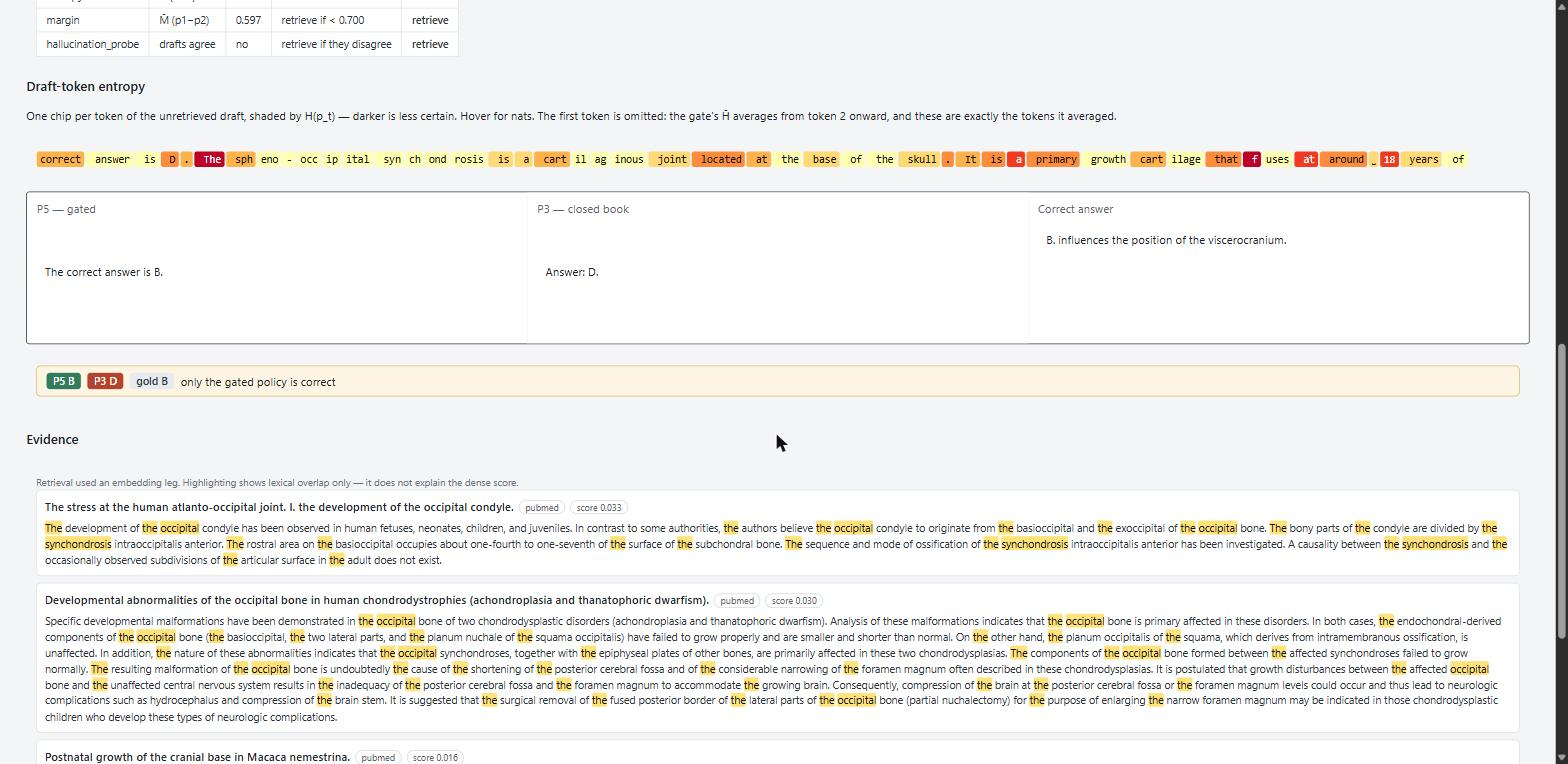
\includegraphics[width=\linewidth]{results/figures/demo/demo_split_verdict.jpg}
  \caption{The interface on a question where the gate changes the outcome. All
    three ensemble members vote to retrieve; the retrieved passages describe
    the spheno-occipital synchondrosis, and the gated policy answers B (gold)
    where closed-book answers D. The strip below the answers is amber rather
    than green precisely because the two policies disagree.}
  \label{fig:demo-split}
\end{figure}

\section{Maintainability and Extension}
\label{sec:impl-maintenance}

The codebase was written on the assumption that someone else would extend it,
so the extension points have to be obvious from the structure rather than from
a document. Adding a gate means implementing the single \texttt{Gate}
interface and naming it in a policy configuration, and the ensemble picks it
up unmodified because it iterates over whatever members it was constructed
with. Adding a model means one YAML file naming the GGUF path, the chat format
and the calibrated thresholds, which is exactly what the two Qwen models
needed. Adding a retriever means implementing the retriever interface and
registering it in the factory. In every case the typed configuration is the
contract, so an invalid extension fails at validation rather than three hours
into a run.

Two conventions support this. No module reaches around the dataclasses to
read another module's internals, so the dependency direction of
Table~\ref{tab:impl-modules} is preserved and any layer can be replaced
wholesale. And anything a future analysis might want is written to the log
rather than computed and discarded, which is why the per-token entropy arrays
and both probe drafts are stored even though neither is needed to produce an
answer. That choice cost disk space, repeatedly saved days of recomputation,
and shaped what Chapter~\ref{ch:eval} was able to ask more than any other
decision in the implementation.